\documentclass[a4paper,14pt]{article}

\usepackage{comment} % Para comentar várias linhas ao mesmo tempo

%matemática
\usepackage{amsmath}
\usepackage{amssymb}

%diagramação
\usepackage{extsizes}
\everymath{\displaystyle}
\usepackage{geometry}
\usepackage{fancyhdr}
\usepackage{multicol}
\usepackage{graphicx}
\usepackage[brazil]{babel}
\usepackage[shortlabels]{enumitem}
\usepackage{cancel}
\usepackage{textcomp}
\usepackage{tcolorbox}

%tabelas
\usepackage{array} % Para melhor formatação de tabelas
\usepackage{longtable}
\usepackage{booktabs}  % Para linhas horizontais mais bonitas
\usepackage{float}   % Para usar o modificador [H]
\usepackage{caption} % Para usar legendas em tabelas
\usepackage{wrapfig} % Para usar tabelas e figuras flutuantes
\usepackage{xcolor} % Para cores do fundo de tabelas
\usepackage{colortbl} % Para cores do fundo de tabelas

%tikzpicture
\begin{comment}
	\usepackage{tikz}
	\usepackage{scalerel}
	\usepackage{pict2e}
	\usepackage{tkz-euclide}
	\usetikzlibrary{calc}
	\usetikzlibrary{patterns,arrows.meta}
	\usetikzlibrary{shadows}
	\usetikzlibrary{external}
\end{comment}


%pgfplots
\usepackage{pgfplots}
\pgfplotsset{compat=newest}
\usepgfplotslibrary{statistics}
\usepgfplotslibrary{fillbetween}

%colours
\usepackage{xcolor}



\columnsep=2cm
\hoffset=0cm
\textwidth=8cm
\setlength{\columnseprule}{.1pt}
\setlength{\columnsep}{2cm}
\renewcommand{\headrulewidth}{0pt}
\geometry{top=1in, bottom=1in, left=0.7in, right=0.5in}

\pagestyle{fancy}
\fancyhf{}
\fancyfoot[C]{\thepage}

\begin{document}
	
	\noindent\textbf{6FMA119, 6FMA120 - Matemática} 
	
	\begin{center}Interpretando dados em gráficos (Versão estudante)
	\end{center}
	
	\noindent\textbf{Nome:} \underline{\hspace{10cm}}
	\noindent\textbf{Data:} \underline{\hspace{4cm}}
	
	%\section*{Questões de Matemática}
	
	\begin{multicols}{2}
	    \noindent \textbf{Gráfico de setores ou de pizza} \\
	    \begin{itemize}
	    	\item Fazer a circunferência e marcar seu centro;
	    	\item Fazer as contas para saber quantos graus correspondem a cada uma das partes (setor);
	    	\item Colocar os ângulos lado a lado na circunferência;
	    	\item Fazer uma legenda e colorir os setores correspondentes.
	    \end{itemize}
	    \textbf{Gráfico de colunas} \\
	    \begin{itemize}
	    	\item Fazer os dois eixos e escolher qual informação vai em cada um deles:
	    	\item Colocar os valores nos eixos;
	    	\item Fazer os retângulos de base unitária e altura conveniente
	    \end{itemize}
	    \textbf{Observação: }o gráfico de barras é o gráfico de colunas com os eixos invertidos.
		\noindent\textsubscript{--------------------------------------------------------------------------}
		\begin{enumerate} 
			\item O gráfico a seguir foi construído a partir de uma pesquisa feita com 50 crianças de 5 a 10 anos. Foi perguntado para cada uma delas qual o doce, entre as seis opções possíveis (chocolate, pirulito, sorvete, bala, chiclete e bolo) que mais gostavam. Observe o resultado: \\\\
			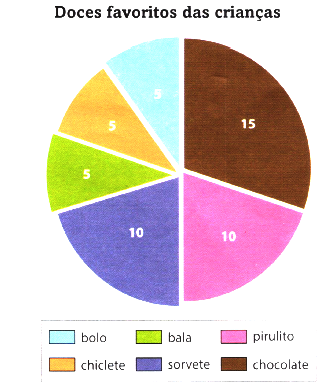
\includegraphics[width=1\linewidth]{6FMA119_imagens/imagem1}
			Fazendo a análise do gráfico, complete as frases:
			\begin{enumerate}[a)]
				\item A fração que corresponde ao número de crianças que preferem chocolate é \underline{~~~~~~~~~~~~~~~~~~~~~~~~~~~~~}.
				\item A fração que corresponde ao número de crianças que preferem pirulito, sorvete ou bala é \underline{~~~~~~~~~~~~~~~~~~~~~~~~~~~~~}.
				\item O ângulo correspondente ao setor das ciranças que preferem chiclete é de \underline{~~~~~~~~~~~~~~~~~~~~~~~~~~~~~}.
				\item O ângulo correspondente ao setor das crianças que preferem bala ou sorvete é de \underline{~~~~~~~~~~~~~~~~~~~~~~~~~~~~~}.
				\item Exatamente metade das crianças preferem sorvete ou \underline{~~~~~~~~~~~~~~~~~~~~~~~~~~~~~}.
			\end{enumerate}	
				\item Foi perguntado para 30 crianças: "Quantas horas por dia você gasta na internet?". As respostas foram as seguintes: 3; 2; 1; 0; 4; 2; 2; 0; 1; 3; 2; 2; 3; 1; 2; 2; 3; 1; 1; 2; 4; 4; 3; 2; 2; 1; 3; 2; 4; 3. Faça o que se pede:
			\begin{enumerate}[a)]
				\item Organize esses dados em uma tabela. \\\\\\\\\\\\\\\\\\\\\\
				\item Passe as informações da tabela para um gráfico de setores ou de pizza. \\\\\\\\\\\\\\\\\\\\\\
				\item Passe as informações da tabela para um gráfico de colunas. \\\\\\\\\\\\\\\\\\\\\\\
			\end{enumerate}
			\item O gráfico a seguir apresenta os desenhos animados preferidos entre 60 crianças no ano de 2019. \\
			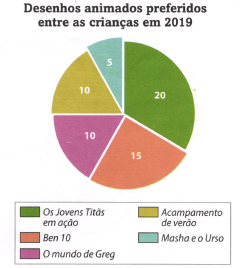
\includegraphics[width=1\linewidth]{6FMA119_imagens/imagem2}
			Responda às questões:
			\begin{enumerate}[a)]
				\item A que fração do total de crianças corresponde cada um de seus setores? \newpage
				\item Quais foram os ângulos utilizados na construção de cada um dos setores? \\\\\\\\\\\\\\
				\item Juntando exatamente 2 desenhos preferidos, podemos ter metade do total de crianças? \\\\\\\\\\\\\\
			\end{enumerate}
			\item Foi feita uma pesquisa com os alunos de uma sala do 6º ano para saber onde passariam as férias de final de ano. O resultado está no gráfico a seguir:
			\\\\\\\\\\\\\\
			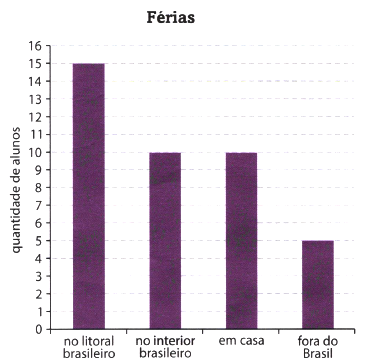
\includegraphics[width=1\linewidth]{6FMA119_imagens/imagem3}
			Analise o gráfico e responda:
			\begin{enumerate}[a)]
				\item Quantos alunos havia na sala de aula em questão? \\\\\\\\\\\\\\
				\item Quantos alunos iriam passar as férias no Brasil? \\\\\\\\\\\\\\
				\item Quantos alunos iriam passar as férias fora de casa? \\\\\\\\\\\\\\
				\item Qual a altura do retângulo que representa o número de alunos que iriam passar as férias fora do Brasil? \\\\\\\\\\\\\\
			\end{enumerate}
			\item Observe o gráfico a seguir.
			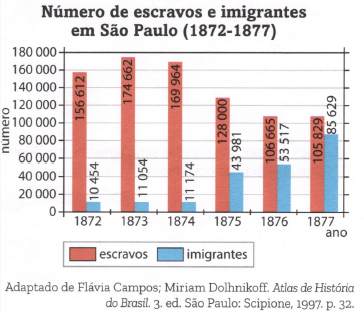
\includegraphics[width=1\linewidth]{6FMA119_imagens/imagem4}
			Com base na análise desse gráfico, é correto afirmar que a razão entre o número de escravos e o número de imigrantes é:
			\begin{enumerate}[a)]
				\item constante no período de 1875 a 1877
				\item crescente no período de 1872 a 1877
				\item decrescente no período de 1872 a 1877
				\item decrescente no período de 1874 a 1877
				\item constante no período de 1873 a 1875
			\end{enumerate}
			%36 a 42
			Para o cálculo da inflação utiliza-se, entre outros, o Índice Nacional de Preços ao Consumidor Amplo (IPCA), que toma como base os gastos das famílias residentes nas áreas urbanas, com rendimentos mensais compreendidos entre um e quarenta salários mínimos. O gráfico a seguir mostra as variações do IPCA de quatro capitais brasileiras no mês de maio de 2008. \\
			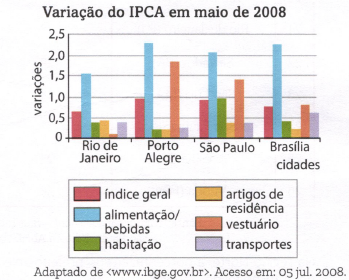
\includegraphics[width=1\linewidth]{6FMA119_imagens/imagem5}
			Com base no gráfico, qual item foi determinante para a inflação de maio de 2008?
			\begin{enumerate}[a)]
				\item Alimentação/bebidas.
				\item Artigos de residência
				\item Habitação.
				\item Vestuário.
				\item Transportes.
			\end{enumerate}
			\item \textit{As empresas querem a metade das pessoas trabalhando o dobro para produzir o triplo.} \\
			\small{Revista Você S/A, 2004.} \\
			Preocupado em otimizar seus ganhos, um empresário encomendou um estudo sobre a produtividade de seus funcionários nos últimos quatro anos, entendida por ele de forma simplificada, como a relação direta entre seu lucro anual (L) e o número de operários envolvidos na produção ($n$). Do estudo, resultou o gráfico a seguir. \\
			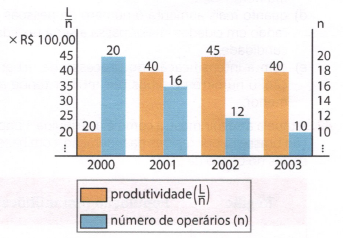
\includegraphics[width=1\linewidth]{6FMA119_imagens/imagem6}
			Ao procurar, no gráfico, uma relação entre seu lucro, produtividade e número de operários, o empresário concluiu que a maior produtividade ocorreu em 2002 e o maior lucro:
			\begin{enumerate}[a)]
				\item em 2000, indicando que, quanto maior o número de operários trabalhando, maior é o seu lucro.
				\item em 2001, indicando que, quanto maior o número de operários não significa necessariamente o aumento dos lucros.
				\item também em 2002, indicando que o lucro e produtividade mantêm uma relação direta que independe o número de operários.
				\item em 2003, devido à significativa redução de despesas com salários e encargos trabalhistas de seus operários.
				\item tanto em 2001 como em 2003, o que indica não haver relação significativa entre lucro, produtividade e número de operários.
			\end{enumerate}
			\item O gráfico a seguir representa a quantidade média de livros que algumas crianças leem por ano. Observe-o e responda ao que se pede:
			\\
			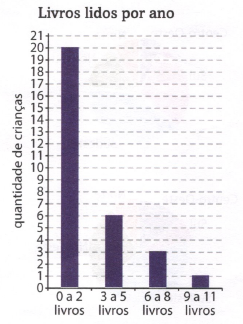
\includegraphics[width=1\linewidth]{6FMA119_imagens/imagem7}
			\begin{enumerate}[a)]
				\item Quantas crianças foram entrevistadas nessa pesquisa? \\\\\\\\
				\item O que podemos afirmar sobre a maioria? \\\\\\\\
				\item Quantas crianças leram 3 ou mais livros? \\\\\\\\
				\item Podemos afirmar quantas crianças não leram livros nesse ano? \\\\\\\\
			\end{enumerate}
			\item Foi feita uma pesquisa sobre os maiores medos de 30 crianças. Observe os resultados no gráfico de setores a seguir: 
			\\
			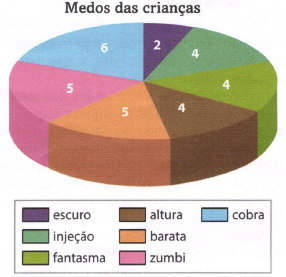
\includegraphics[width=1\linewidth]{6FMA119_imagens/imagem8}
			\begin{enumerate}[a)]
				\item Monte uma tabela que represente os mesmos resultados dos gráficos. \\\\\\\\\\\\\\\\\\\\\\\\
				\item Qual o medo da maioria das crianças em questão? \\\\\\\\
				\item Qual o ângulo que determina o setor representante do "medo de injeção"? \\\\\\\\
			\end{enumerate}
			\item (Enem) Os dados a seguir referem-se à origem do petróleo consumido no Brasil em dois diferentes anos. \\
			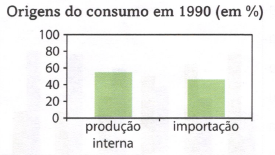
\includegraphics[width=1\linewidth]{6FMA119_imagens/imagem9}
			\\
			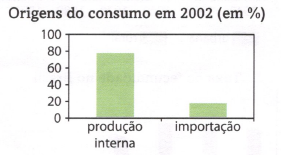
\includegraphics[width=1\linewidth]{6FMA119_imagens/imagem10}
			\\
			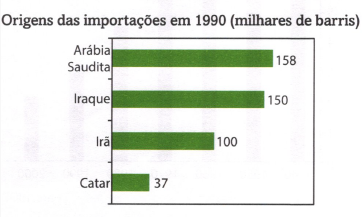
\includegraphics[width=1\linewidth]{6FMA119_imagens/imagem11}
			\\
			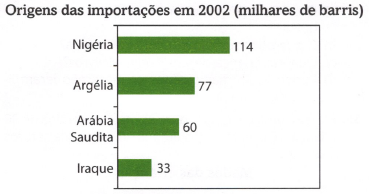
\includegraphics[width=1\linewidth]{6FMA119_imagens/imagem12}
			Analisando os dados, pode-se perceber que o Brasil adotou determinadas estratégias energéticas, dentre as quais podemos citar:
			\begin{enumerate}[a)]
				\item a diminuição das importações dos países muçulmanos e redução do consumo interno.
				\item a redução da produção nacional e diminuição do consumo do petróleo produzido no Oriente Médio.
				\item a redução da produção nacional e o aumento das compras de petróleo dos países árabes e africanos.
				\item o aumento da produção nacional e redução do consumo de petróleo vindo dos países do Oriente Médio.
				\item o aumento da dependência externa de petróleo vindo de países mais próximos do Brasil e redução do consumo interno.
			\end{enumerate}
			\item (Enem) Ao longo do século XX, as características da população brasileira mudaram muito. Os gráficos mostram as alterações na distribuição da população da cidade e do campo e na taxa de fecundidade (número de filhos por mulher) no período entre 1940 e 2000.
			\\
			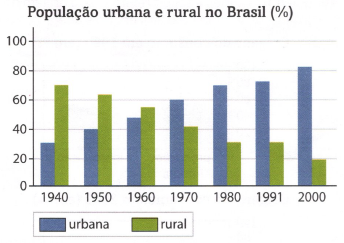
\includegraphics[width=1\linewidth]{6FMA119_imagens/imagem13}
			\\
			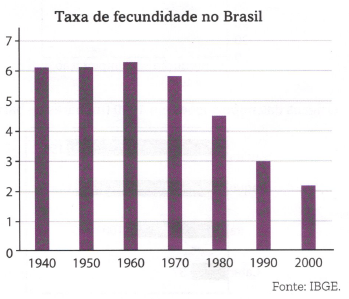
\includegraphics[width=1\linewidth]{6FMA119_imagens/imagem14}
			Comparando-se os dados dos gráficos, pode-se concluir que:
			\begin{enumerate}[a)]
				\item o aumento relativo da população rural é acompanhado pela redução da taxa de fecundidade.
				\item quando predominava a população rural, as mulheres tinham em média três vezes menos filhos do que hoje.
				\item a diminuição relativa da população rural coincide com o aumento do número de filhos por mulher.
				\item quanto mais aumenta o número de pessoas morando em cidades, maior passa a ser a taxa de fecundidade.
				\item com a intensificação do processo de urbanização, o número de filhos por mulher tende a ser menor. \newpage
			\end{enumerate}
			\item A tabela a seguir mostra como é distribuída a população brasileira por regiões da federação, com base em dados do Censo de 2010.
			\begin{table}[H]
				\begin{tabular}{|p{3.5cm}|p{3.5cm}|}
					\hline
					\textbf{Região} & \textbf{População (em milhões)}  \\ \hline
					Norte & 15,8  \\ \hline
					Nordeste & 53,0 \\ \hline
					Sudeste & 80,3 \\ \hline
					Sul & 27,3 \\ \hline
					Centro-Oeste & 14,0  \\ \hline
				\end{tabular}
			\end{table}
			Qual dos gráficos de setores a seguir melhor representa os dados dessa tabela?
			\\
			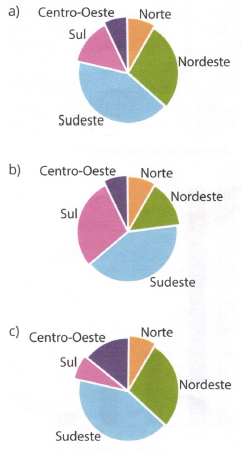
\includegraphics[width=1\linewidth]{6FMA119_imagens/imagem15}
			\\
			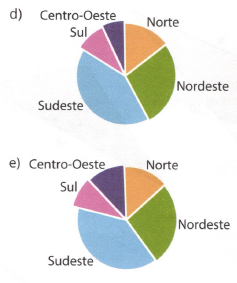
\includegraphics[width=1\linewidth]{6FMA119_imagens/imagem16}
		\end{enumerate}
		$~$ \\ $~$ \\ $~$ \\ $~$ \\ $~$ \\ $~$ \\ $~$ \\ $~$ \\ $~$ \\ $~$ \\ $~$ \\ $~$ \\ $~$ \\ $~$ \\ $~$ \\ $~$ \\ $~$ \\ $~$ \\ $~$ \\ $~$ \\ $~$ \\ $~$ \\ $~$ \\ $~$ \\ $~$ \\ $~$ \\ $~$
	\end{multicols}
\end{document}